%======================================================================
\chapter{Cross-Domain Sentence Modeling for Relevance Transfer}
%======================================================================
\label{ch:model}

%\myworries{Go into details of BERT, then how we use it...}
%\myworries{Maybe give example for how BERT for relevance modeling looks like? Input? May draw my own diagram}
%\myworries{Can I add some math-y stuff to describe what BERT is doing?}

Our model is based on sentence-level relevance modeling and document re-ranking with BERT.
By training BERT as a relevance classifier, we aim to extract valuable semantic matching signals which can be leveraged to re-rank a list of candidate documents retrieved with a term-matching technique such as BM25.
We also explore applying cross-domain relevance transfer to exploit models of relevance learned on out-of-domain collections, which is crucial in re-ranking documents that are too long for BERT to directly process.
This chapter introduces the datasets that we use to fine-tune our relevance model and to evaluate them on end-to-end document retrieval, and describes the details of our BERT-based sentence-level relevance classifier and document re-ranker.

\section{Datasets}

\subsection{Fine-Tuning}

In order to model sentence-level relevance with BERT, we need training pairs of queries and short text, annotated with relevance labels.
Fortunately, a number of collections fortuitously contain such relevance judgments at the sentence and passage level, which makes them the ideal choice for training our models.
We fine-tune BERT on three such sentence- and passage-level datasets individually and in combination:\ TREC Microblog~\cite{ounisoverview}, MicroSoft MAchine Reading Comprehension~\cite{nguyen2016msmarco} and TREC Complex Answer Retrieval~\cite{dietz2017trec}.
The details of each dataset are provided below.

\subsubsection{TREC Microblog (MB)}

\begin{figure}[t!]
	\begin{framed}
%		\centering
    		\textbf{Query:} bbc world service staff cuts \\
    		\textbf{Text:} irish times : bbc world service confirms cuts : the bbc world service will shed around 650 jobs or more \\
    		\textbf{Relevance:} 1 (``relevant'')
	\end{framed}
\label{mb-example}
 \caption{A sample query and relevant tweet pair from the MB dataset.}
\end{figure}

\begin{table}[t]
\vspace{0.2cm}
\centering
\begin{tabular}{lccc}
\toprule
\textbf{Type} \mbox{\hspace{0.5cm}} & \textbf{Training Set} \mbox{\hspace{1.0cm}} & \textbf{Validation Set} \mbox{\hspace{1.0cm}} \\
\toprule
Number of queries & 166 & 59 \\
Number  of tweets & 133K & 44K  \\
%Percentage of relevant tweets  & 7\% & 16\%  \\
\bottomrule
\end{tabular}
\vspace{0.2cm}
\caption{Statistics about the MB dataset.}
\label{tab:mb-stats}
%\vspace{-0.6cm}
\end{table}

The TREC Microblog dataset draws from the Microblog Tracks at TREC from 2011 to 2014, with topics and relevance judgments over tweets.
Topics associated with tweets are treated as queries, and each of the four datasets contains approximately 50 queries.
The nature of this collection differs from newswire documents that we evaluate our models on in distinct ways:\
first of all, tweets have much fewer tokens than newswire documents.
By definition, tweets are limited to 280 characters.
%The length distribution of tweets in MB is displayed in \Figure X}.
Furthermore, because queries and tweets in this dataset are comparable in length, exact matches of query terms occur less frequently in the tweets than they might in longer documents such as news articles.
Therefore, semantic matching signals may take precedence in improving retrieval effectiveness on MB.
%\myworries{How is this relevant to our training? It's valuable because...}
Related to this point, tweets are expressed in a much less formal language than news articles.
Tweets may characteristically contain various abbreviations (partly due to the aforementioned length constraint), informal conventions such as hashtags or typos; such informal language may result in term mismatches in the case of exact matching.
It may therefore be helpful to catch other semantic signals with a deep neural network.

We use the MB data\footnote{\url{https://github.com/jinfengr/neural-tweet-search}} prepared by Rao et al.~\cite{rao2019tweet}.
We extract the queries, tweets and relevance judgments from the dataset, excluding metadata such as query time and URLs of the tweets.
Both queries and tweets are segmented into token sequences.
Relevance judgments in MB are reported on a three-point scale, i.e., (``non-relevant'', ``relevant'' and ``highly relevant''), however, for the purposes of this work we treat both higher degrees of relevance as equal~\cite{ounisoverview}.
We sample 25\% of the data for the validation set, and use the rest for fine-tuning BERT.
%We experiment with different splits, and find this split to be ideal.

\subsubsection{MicroSoft MAchine Reading Comprehension (MS MARCO)}

\begin{table}[b]
\vspace{0.2cm}
\centering
\begin{tabular}{lccc}
\toprule
\textbf{Type} \mbox{\hspace{0.5cm}} & \textbf{Training Set} \mbox{\hspace{1.0cm}} & \textbf{Validation Set} \mbox{\hspace{1.0cm}} \\
\toprule
Number of queries & 809K & 6.9K \\
Number  of passages & 12.M & 6.9M \\
%Percentage of relevant passages  & asd & asd \\
\bottomrule
\end{tabular}
\vspace{0.2cm}
\caption{Statistics about the MS MARCO dataset.}
\label{tab:marco-stats}
\end{table}

\begin{figure}[b!]
	\begin{framed}
%		\centering
    		\textbf{Query:} is a little caffeine ok during pregnancy \\
    		\textbf{Relevant Passage:} We don't know a lot about the effects of caffeine during pregnancy on you and your baby. So it's best to limit the amount you get each day. If you're pregnant, limit caffeine to 200 milligrams each day. This is about the amount in 1.5 8-ounce cups of coffee or one 12-ounce cup of coffee. \\
    		\textbf{Non-relevant Passage:} It is generally safe for pregnant women to eat chocolate because studies have shown to prove certain benefits of eating chocolate during pregnancy. However, pregnant women should ensure their caffeine intake is below 200 mg per day. \\
	\end{framed}
\label{marco-example}
 \caption{A sample relevant and non-relevant passage pair for a query from the MB dataset}
\end{figure}

MS MARCO is a large-scale machine reading comprehension and question answering dataset that is extensively used in the NLP community.
MS MARCO~\cite{nguyen2016msmarco} features user queries sampled from Bing’s search logs and passages extracted from web documents.
The dataset is composed of tuples of a query associated with a relevant and non-relevant passage.
On average, each query has one relevant passage.
However, some may have no relevant passage at all as the dataset is constructed from the top 10 passages manually annotated by human judges.
Therefore, some relevant passages might not have been retrieved with BM25.
%\myworries{Rephrase this}
MS MARCO can be distinguished from similar datasets by its size and real-world nature.
Similar to MB, MS MARCO is representative of a natural, and noisy, distribution of information needs, unlike other datasets that often contain high-quality text that may not reflect the use in real life.
%\myworries{What else? Robust systems}

Here we focus on the passage-ranking dataset of MS MARCO.
Following the settings in Nogueira et al.~\cite{nogueira2019passage}, we train BERT on approximately 12.8M training samples.
The development set is composed of approximately 6.9K queries, each paired with the top 1000 most relevant passages in the MS MARCO dataset as retrieved with BM25.
Similarly, the evaluation set contains approximately 6.8K queries and their top 1000 passages, but without the relevance annotations.
%The models in Section \myworries{X} were trained on less than 2\% of the total training set (~12.8M) due to the size of the dataset and time required to train on it even on TPUs.
%According to Nogueira et al. \cite{nogueira2019passage}, training for up to 12.5\% of the total data does not improve MRR@10 on the validation set.
%\myworries{Maybe remove MRR, and better transition}

\subsubsection{TREC Complex Answer Retrieval (CAR)}

\begin{table}[b!]
\vspace{0.2cm}
\centering
\begin{tabular}{lccc}
\toprule
\textbf{Type} \mbox{\hspace{0.5cm}} & \textbf{Training Set} \mbox{\hspace{1.0cm}} & \textbf{Validation Set} \mbox{\hspace{1.0cm}} \\
\toprule
Number of queries & 3M & 700K \\
Number of passages & 30M & 7M \\
\bottomrule
\end{tabular}
\vspace{0.2cm}
\caption{Statistics about the CAR dataset.}
\label{tab:car-stats}
\end{table}

%\begin{figure}[b!]
%	\begin{framed}
%		\centering
%    		\textbf{Query:} bbc world service staff cuts \\
%    		\textbf{Text:} irish times : bbc world service confirms cuts : the bbc world service will shed around 650 jobs or more \\
%    		\textbf{Relevance:} 1 (``relevant'')
%	\end{framed}
%\label{car-example}
% \caption{\myworries{TODO}}
%\end{figure}

TREC CAR \cite{dietz2017trec} uses paragraphs extracted from all of the English Wikipedia, except the abstracts.
Each query is formed by concatenating an article title and a section heading, with all passages under that section considered relevant.
The goal of this track is to automatically collect and condense information for a complex query into a single coherent summary; the priority is aggregating synthesized information in the form of references, facts, and opinions.
However, CAR is a synthetic dataset in the sense that queries and documents do not reflect real-world distributions or information needs.
Manual annotations for only the top 5 passages retrieved are provided, meaning some relevant passages may not be annotated if they rank lower.
For this reason, we opt to use automatic annotations that provide relevance judgments for all possible query-passage pairs.
%\myworries{More?}

The dataset has five predefined folds over the queries.
Paragraphs corresponding to the first four folds are used to construct the training set consisting of approximately 3M queries, and the rest the validation set of around 700K queries.
The training pairs are generated by retrieving the top 10 passages with BM25.
%The original test set used to evaluate submissions to TREC CAR is used for testing purposes.
A subtle detail to note is that the official BERT models are pre-trained on the entire Wikipedia dump; therefore, they have also been trained on documents in the TREC CAR test collection albeit in an unsupervised fashion.
In order to avoid the leak of test data into training, we use the BERT model pre-trained only on the half of Wikipedia present in CAR training samples~\cite{nogueira2019passage}.
%30M fine-tuning query-passage pairs were generated by retrieving the top 10 passages from the entire CAR corpus with BM25.
%Similar to MS MARCO, training on more than 40\% of the training set did not lead to any improvements on the validation set

\subsection{Evaluation}

We conduct end-to-end document ranking experiments on three TREC newswire collections:\ the Robust Track from 2004 (Robust04)~\cite{Voorhees_TREC2004_robust} and the Common Core Tracks from 2017 and 2018 (Core17~\cite{allan2017trec} and Core18~\cite{core2018trec}).

\subsubsection{Robust04}

Robust04 draws from the set of documents in TREC Disks 4 and 5, spanning news articles from Financial Times and LA Times, except the Congressional Record.
The collection comprises 250 topics, with relevance judgments over 500K documents.
The goal of the Robust track is to improve the consistency and robustness of retrieval methods by focusing ``ad hoc'' search on poorly performing topics~\cite{Voorhees_TREC2004_robust}.
%The task involves searching across a fixed set of documents using previously unseen topics.
Notably the distribution of document lengths in Robust04 is highly skewed, with the majority of documents having fewer than 2K tokens and a couple of documents having more than 10K tokens.
%Existing neural re-rankers such as DRMM~\cite{guo2016deep} and KNRM~\cite{xiong2017knrm} are known to struggle with documents in the tail of the distribution.

\subsubsection{Core17 \& Core18}

Core17 and Core18 build on the TREC 2017 and 2018 Common Core Tracks, respectively.
The motivation behind these tracks is to build up-to-date test collections based on more recently created documents.
%\myworries{that avoids the pitfalls of depth-k pooling}
Core17 contains 1.8M articles from the New York Times Annotated Corpus while Core18 has around 600K articles from the TREC Washington Post Corpus.
Core17 and Core18 have only 50 topics each, which are drawn from the Robust Track topics.
Given their relatively recent release, literature on these collections is still sparse.

\section{Modeling Relevance with BERT}

We propose modeling sentence-level and passage-level relevance with BERT to capture semantic signals helpful for relevance prediction.
%\myworries{Better alternative to capture semantic signals?}
This approach is motivated by the application of fine-tuning in NLP where a large transformer model trained for language modeling can be used for various downstream tasks.
In our implementation, we choose BERT as our base mode.
BERT is trained on copious amounts of unsupervised data from the Google BookCorpus and English Wikipedia with masked language modeling.
%\myworries{Talk about relevance prediction too}
Although the training procedure does not involve any explicit objective to extract linguistic features, it has been shown to implicitly recognize such features as subject-verb agreement and conference resolution~\cite{jawahar2019does, clark2019does}, which allows a number of NLP tasks to greatly benefit from features implicitly encoded in BERT weights.

\subsection{Relevance Classifier}

The core of our model is a BERT-based sentence-level relevance classifier.
In other words, we build a model on top of BERT to predict a relevance score $ s_i $ for a sentence or passage $ d_i $ given a query $ q $.
Because the maximum input length that BERT can handle is 512 tokens, we limit our training data to sentence-level and passage-level datasets.
In other words, $ d_i $ are either tweets drawn from TREC Microblog or passages from MS MARCO or TREC CAR.
Following Nogueira et al.~\cite{nogueira2019passage}, we frame relevance modeling as a binary classification task.
%Figure \myworries{X} illustrates how BERT can be used for to predict the relevance of a given sentence.
%\myworries{Add diagram to explain the relevance modeling process}
More specifically, we feed query-text pairs into the BERT model with their respective relevance judgments (i.e., 0 for non-relevant and 1 for relevant).
Through this training process BERT learns to estimate the relevance of an unseen text for a given query.
The details of the input representation to BERT and specifics of fine-tuning BERT for relevance prediction are discussed at length in the remainder of this chapter.

\subsection{Input Representation}

%\begin{figure}[t!]
%	\begin{framed}
%		\centering
%		blahblahblah
%	\end{framed}
%\label{bert-tokenization-example}
% \caption{\myworries{Put tokenized BERT input example?}}
%\end{figure}

\begin{figure}[t!]
\centering
  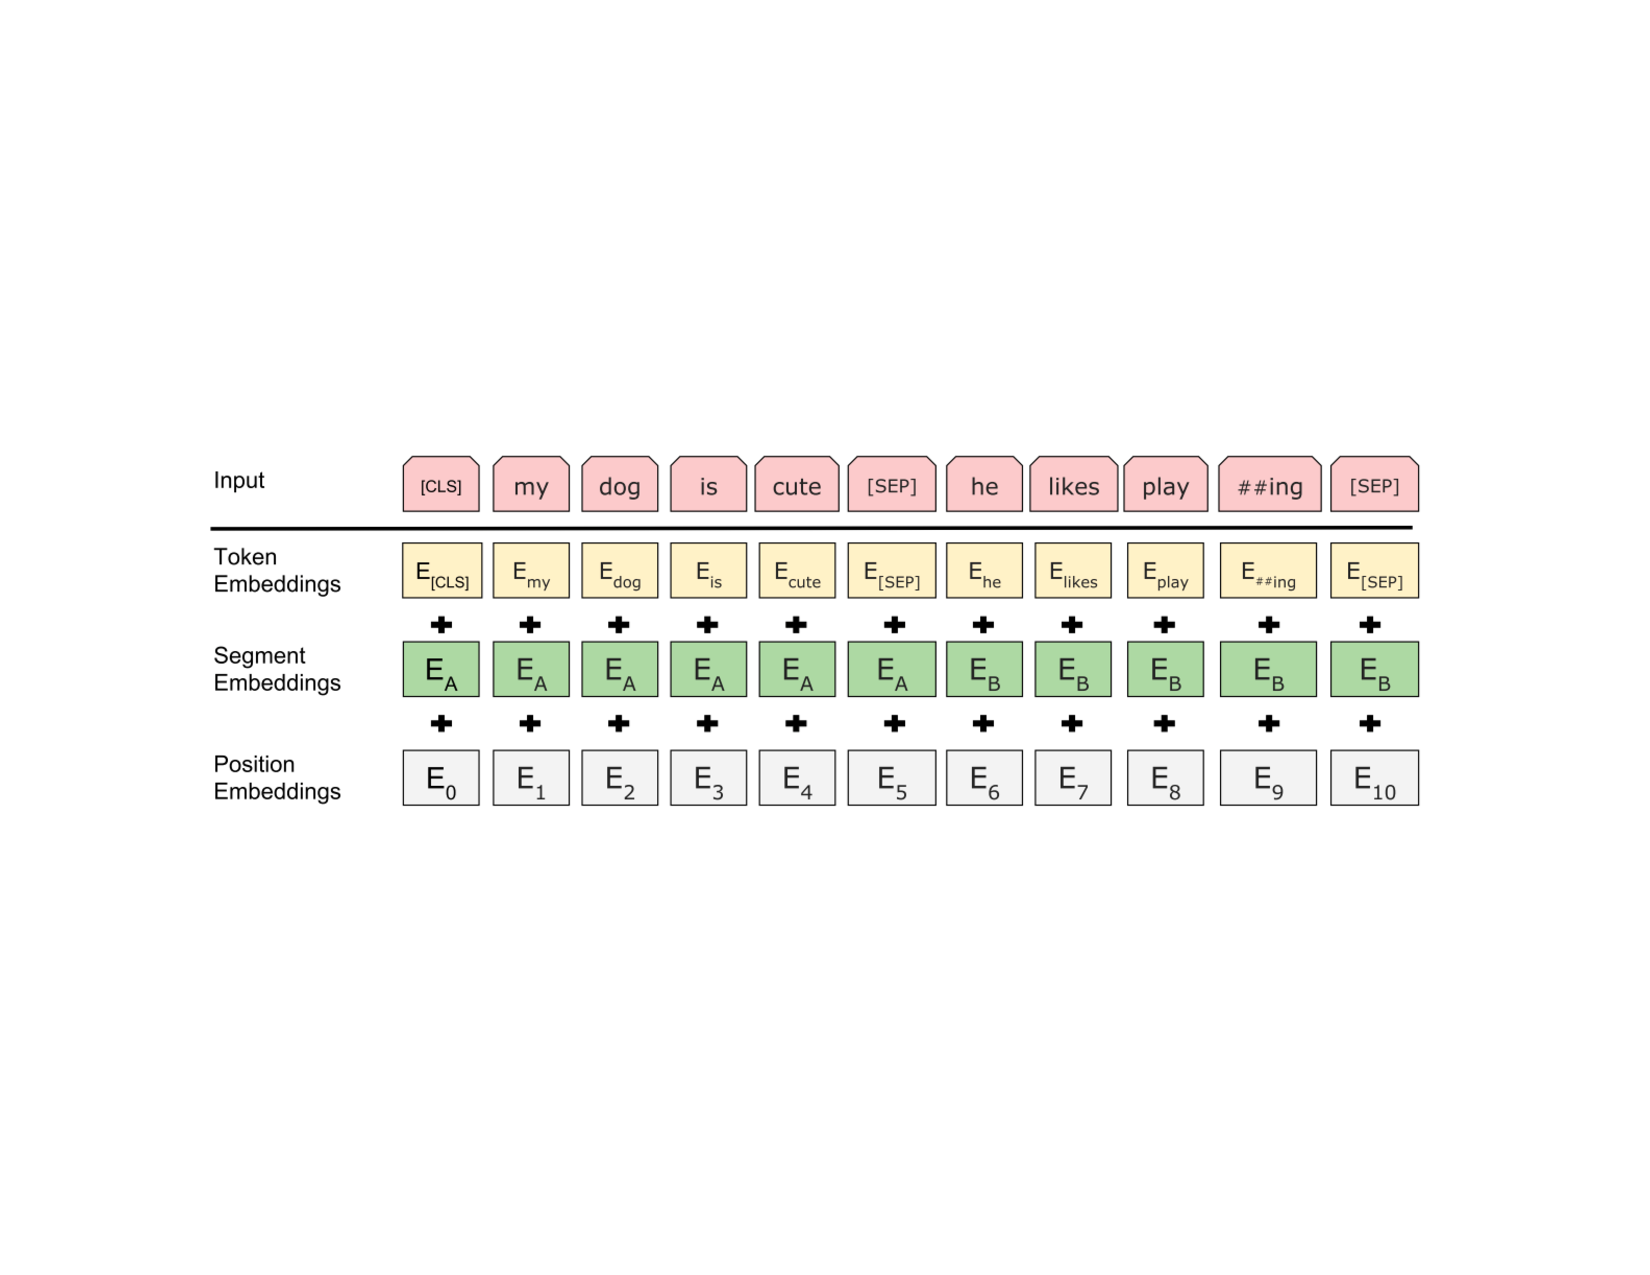
\includegraphics[width=6.5in]{figures/input.pdf}
\caption{Illustration of BERT input representation adapted from Devlin et al.~\cite{devlin2018bert}.}
\label{fig:bert_input}
\end{figure}

We form the input to BERT by concatenating the query $ q $ and a sentence $ d $ into the sequence [\texttt{[CLS]}, $q$, \texttt{[SEP]}, $d$, \texttt{[SEP]}] .
The \texttt{[SEP]} metatoken is used to distinguish between two non-consecutive token sequences in the input, i.e., query and text, and the \texttt{[CLS]} signifies a special symbol for classification output.
Although BERT supports variable length token sequences, the final input length must be consistent across each batch.
Therefore, we pad each sequence in a mini-batch to the maximum length in the batch.

The complete input embeddings of BERT are comprised of token, segmentation, and position embeddings.
The first is constructed by tokenizing the above sequence with the proper metatokens in place with the BERT tokenizer.
Since BERT was trained based on WordPiece tokenization, we use the same tokenizer to achieve optimal performance.
WordPiece tokenization may break words into multiple subwords in order to more efficiently deal with out-of-vocabulary words and better represent complex words.
During training, the subwords derived with WordPiece tokenization are reconstructed based on the training corpus.
After tokenization, each token in the input sequence is converted into token IDs corresponding to the index in BERT's vocabulary.
Tokens that do not exist in the vocabulary are represented with a special \texttt{[UNK]} token.

The segment embeddings indicate the start and end of each sequence, whether it be a single sequence or a pair.
For relevance classification where we have two texts in the input sequence, i.e., query and sentence, the segment embeddings corresponding to the tokens of the first sequence, i.e., the query, are all 0's, and those for the second sequence, i.e., the document, are all 1's.
The position embeddings are learned for sequences up to 512 tokens, and help BERT recognize the relative position of each token in the sequence.
The input representation for a sample short query-sentence pair is shown in Figure \ref{fig:bert_input}.

%An example BERT input for MB is shown in Figure \myworries{X}.
%\myworries{Example with complex words}

\subsection{Fine-Tuning}

%\myworries{Go more into detail about NN stuff?}
A variety of useful deep semantic features are already encoded in pretrained BERT weights.
It is thus possible to fine-tune BERT for a specific downstream task with less data and time by adding a fully-connected layer on top of the network.
Intuitively, the lower layers of the network have already been trained to capture latent features relevant to the task.

To fine-tune BERT for relevance modeling, we append a single layer neural network to BERT for classification.
This layer consists of $ K \times H $ randomly initialized neurons where $ K $ is the number of classifier labels and $ H$ is the hidden state size.
For relevance classification, we have two labels indicating whether the sentence is relevant or non-relevant for the given query ($ K = 2 $).

The final hidden state corresponding to the first token, i.e., \texttt{[CLS]}, provides a $ H $-dimensional aggregate representation of the input sequence that can be used for classification.
We feed the final hidden state in the model corresponding to \texttt{[CLS]} into the classification layer.
The probability that the sentence $ d_i $ is relevant to the query $ q_i $ is thus computed with standard softmax:
 
\begin{equation}
\sigma (y_i) = \frac{e^{y_i}}{\sum_j e^{y_j}}
\end{equation}

\noindent where $\sigma (y_i)$ maps the arbitrary real value $ y_i $ into a probability distribution.
Intuitively, $\sigma (y_i)$ represents the relevance score for the sentence $ d_i $.
The parameters of BERT and the additional softmax layer are optimized jointly to maximize the log-probability of the correct label with cross-entropy loss.

\section{Re-ranking with BERT}

%\begin{figure}[b!]
%\centering
%  \includegraphics[width=4in]{bert_real.png}
%\caption{...}
%\label{fig:bert_real}
%\end{figure}

Fine-tuning BERT on relevance judgments of query-text pairs allows us to obtain a model of relevance so that we can compute sentence-level relevance scores easily on any collection.
However, recall that we train BERT on sentence-level or passage-level datasets so as not to exceed the maximum input size of BERT.
These training datasets come from very different distributions than the test collections introduced in Chapter~\ref{ch:results}.
In order to predict relevance on much longer newswire documents, we explore cross-domain relevance transfer by using models trained on MB, MS MARCO and CAR on newswire collections.
Our hypothesis is that if a neural network with a large capacity such as BERT can capture relevance in one domain, the model of relevance might successfully transfer to other domains.
%\myworries{Probably need a couple more sentences to make this more coherent}

To apply cross-domain relevance transfer, we retrieve relevant documents from the collection to depth 1000 with BM25 and split each document into its constituent sentences to match the input size of BERT.
We then run inference over the sentences with our models fine-tuned on out-of-domain datasets to compute a score for each sentence.
We determine overall document scores by combining exact and semantic matching signals.
Based on BM25+RM3 document scores we know a ranking of documents based on exact matches of query terms.
Sentence-level scores obtained with BERT reveal other implicit semantic information not evident to BM25.
By combining the two sets of relevance matching signals, we establish a more diverse notion of relevance, leading to a better ranking of documents.
%\myworries{Give example diagram of sentence score ranking? Maybe with BM25?}

%Using either set of scores to rank documents neglects crucial information from the other, so we interpolate the scores 
Therefore, to determine overall document relevance, we combine the top $ n $ scores with the original document score as follows:
\begin{equation} \label{eq:1}
s_f = \alpha \cdot s_{doc}  + (1 - \alpha) \cdot \sum_{i = 1}^n w_i \cdot s_i
\end{equation}

\noindent where $ s_{doc} $ is the original document score and $ s_i $ is the $ i $-th top scoring sentence according to BERT.
In other words, the relevance score of a document comes from the combination of a document-level term-matching score and relevance evidence contributions from the top sentences in the document as determined by BERT.

We experiment with the number of top scoring sentences to consider while computing the overall score, and find that using only the top 3 sentences is often enough.
In general, considering any more does not yield better results.
To tune hyperparameters $ \alpha $ and the $ w_i $'s  in Equation~\ref{eq:1}, we apply five-fold cross-validation over TREC topics.
For Robust04, we follow the five-fold cross-validation settings in Lin~\cite{lin2019neural} over 250 topics.
For Core17 and Core18 we similarly apply five-fold cross validation.
We learn parameters $\alpha$ and the $w_i$ on four folds via exhaustive grid search with $ w_1 = 1 $ and varying $ \alpha, w_2, w_3 \in [0, 1] $ with a step size 0.1, selecting the values that yield the highest AP on the remaining fold.

\section{Experimental Setup}

\subsection{Training and Inference with BERT}

We fine-tune $ \textrm{BERT}_{\textrm{\scriptsize Large}} $~\cite{devlin2018bert} on the datasets introduced earlier in this section:\ TREC Microblog, MS MARCO, and TREC CAR.
In our implementation we adopt the interface \texttt{BertForNextSentencePrediction} corresponding to $ \textrm{BERT}_{\textrm{\scriptsize Large}} $ from the Huggingface \texttt{transformers} (previously known as \texttt{pytorch-pretrained-bert}) library\footnote{\url{https://github.com/huggingface/transformers}} as our base model.
The maximum sequence length, i.e., 512 tokens, is used for BERT in all our experiments.

The fine-tuning procedure introduces few new hyperparameters in addition to those already used in pre-training:\ batch size, learning rate, and number of training epochs.
Due to the large amount of training data in MS MARCO and TREC CAR, BERT is initially trained on Google's TPU's with a batch size of 32 for 400k iterations.
% following ~\cite{nogueira2019passage}.
We use Adam \cite{kingma2014adam} with an initial learning rate of $ 3 \times 10^{-6}$, $ \beta_1 = 0.9 $ and $ \beta_2 = 0.999 $ and L2 decay of 0.01.
Learning rate warmup is applied over the first 10K steps with linear decay of learning rate.
We apply dropout with probability of 0.1 across all layers.

We train all other models using cross-entropy loss for 5 epochs with a batch size of 16.
We conduct all our experiments on NVIDIA Tesla P40 GPUs with PyTorch v1.2.0.
We use the Adam optimizer \cite{kingma2014adam} with an initial learning rate of $ 1 \times 10^{-5}$, linear learning rate warmup at a rate of 0.1 and decay of 0.1.
We find that applying diminishing learning rates is especially important in fine-tuning BERT in order to preserve the information encoded in the original BERT weights and speed up training.

%\subsection{Evaluation}
\subsection{End-to-End Document Retrieval}

We retrieve an initial ranking of 1000 documents for each query in Robust04, Core17, and Core18 using the open-source Anserini information retrieval toolkit based on Lucene 8.
To ensure fairness across all three collections, we use BM25 with RM3 query expansion with default parameters.
Before running inference with BERT to obtain relevance scores, we preprocess the retrieved documents:\
first, we clean the documents by stripping any HTML/XML tags and split each document into its constituent sentences with NLTK's Stanford Tokenizer.\footnote{\url{https://nlp.stanford.edu/software/tokenizer.shtml}}
If the length of a sentence with the meta-tokens still exceeds the maximum input length of BERT, we further segment the spans into fixed sized chunks.
%Candidate documents are re-ranked based on the combination of BM25 and sentence scores computed with BERT according to Equation~\ref{eq:1} with the hyperparameters optimized on
In order to make our results comparable to the baselines and consistent with the literature, we report retrieval effectiveness in terms of AP, P@20, and NDCG@20.

%\section{Evaluation Metrics}
%
%Evaluation in information retrieval relies on the distinction between ``relevant'' and ``irrelevant'' documents with respect to an information need as expressed by a query.
%A number of automatic evaluation metrics has been formalized specifically for ranking tasks, some of which are described below.
%
%%The size of most document collections makes it infeasible for humans to manually judge the relevance of all documents.
%%All relevant documents need to be labelled to prevent false negatives, i.e: treating documents which are in fact relevant as irrelevant.
%
%\smallskip \noindent {\bf Mean Average Precision (MAP)}
%
%Precision specifies what fraction of a set of retrieved documents is in fact relevant for a given query $ q $.
%By extension, average precision (AP) expresses the average of the precision values obtained for the set of top $ k $ documents for the query.
%Support that $ D = \{d_1, ..., d_{m_j}\} $ is the set of all relevant documents for a query $ q_j $, then AP can be formulated as:
%
%\begin{equation}
%AP = \frac{1}{m_j} \sum^{m_j} _{k = 1} P(R_{jk})
%\end{equation}
%
%\noindent where $ R_{jk} $ represents the set of top $ k $ ranked retrieval results.
%
%The respective AP for each query $ q_{j} \in Q $ can be aggregated to obtain mean average precision (MAP) for the overall retrieval effectiveness in the form of an aggregate measure of quality across all topics:
%
%\begin{equation}
%MAP = \frac{\sum^{|Q|} _{j = 1} AP}{Q} = \frac{1}{Q} \sum^{|Q|} _{j = 1} \frac{1}{m_j} \sum^{m_j} _{k = 1} P(R_{jk})
%\end{equation}
%
%%\myworries{Meaning of MAP: To recapitulate, if the AP is 0.5, the relevant
%%answer occurs at every second position. If the AP score is 0.3, the relevant answer occurs
%%at every 3rd position and an AP score of 0.1 would mean that every 10th answer is correct.}
%
%\noindent MAP is known to have especially good discrimination and stability compared to other evaluation metrics, which makes it the ideal choice for large text collections~\cite{manning2010introduction}.
%It is hence one of the standard metrics among the TREC community.
%
%\smallskip \noindent {\bf Precision at k (P@k)}
%
%While MAP factors in precision at all recall levels, certain applications may have a distinctly different notion for ranking quality.
%Particularly in the case of web search, the user often only cares about the results on the first page or two.
%This restriction essentially requires measuring precision at fixed low levels of retrieved results, i.e., top $ k $ documents -- hence the name for the metric ``precision at $ k $''.
%On the one hand, it eliminates the need for any estimate of the size of the set of relevant documents because it is only concerned with the top documents.
%However, it also produces the least stable results out of all evaluation metrics.
%Moreover, precision at $ k $ does not average well because it is too sensitive to the total number of relevant documents for a query.
%
%\smallskip \noindent {\bf Normalized Discounted Cumulative Gain (NDCG@k)}
%
%Cumulative gain (CG) simply computes the sum of relevance labels for all the retrieved documents, treating the search results as an unordered set.
%However, since a highly relevant document is inherently more useful when it appears higher up in the search results, CG has been extended to discounted cumulative gain (DCG).
%DCG estimates the relevance of a document based on its rank among the retrieved documents.
%The relevance measure is accumulated from top to bottom, discounting the value of documents at lower ranks.
%NDCG at $ k $ measures DCG for the top $ k $ documents, normalizing by the highest possible value for a query; therefore, a perfect ranking yields NDCG equals 1.
%
%NDCG is uniquely useful in applications with a non-binary notion of relevance, e.g: a spectrum of relevance.
%This makes NDCG comparable across different queries:\
%The NDCG values for all queries can be averaged to reliably evaluate the effectiveness of a ranking algorithm for various information needs across a collection.
%Given a set of queries $ q_j \in Q $ and relevance judgements $ R_{dj} $ for a document $ d $:\
%
%\begin{equation}
%NDCG(Q, k) = \frac{1}{|Q|} \sum ^{|Q|} _{j = 1} Z_{kj} \sum ^k _{m = 1} \frac{2^{R_{jm}} - 1}{log_2 (1 + m)'}
%\end{equation}
%
%\noindent where $ Z_{kj} $ is the normalization factor.